\documentclass[14pt,a4paper]{scrartcl}
\usepackage{cmap}
\usepackage[utf8]{inputenc}
\usepackage[T1,T2A]{fontenc}
\usepackage[english,russian]{babel}
\usepackage{relsize}
\usepackage{graphicx}
\usepackage{subfigure}
\usepackage{mathtools}
\usepackage{amssymb}
\usepackage{float}
\usepackage{sidecap}
\usepackage{wrapfig}
\usepackage{caption}
\usepackage[table,xcdraw]{xcolor}
\usepackage{listings}
\usepackage{minted}
\usepackage{multirow}
\usepackage{bigstrut}
\begin{document}
	\begin{titlepage}
	\begin{center}
		\large
		МИНИСТЕРСТВО ОБРАЗОВАНИЯ И НАУКИ\\ РОССИЙСКОЙ ФЕДЕРАЦИИ
		
		\vspace{0.5cm}
		
		МГТУ им Н.Э.Баумана
		\vspace{0.25cm}
		
		Факультет ФН
		
		Кафедра вычислительной математики и математической физики
		\vfill
		
		
		Соколов Арсений Андреевич\\
		\vfill
		
		
		{\LARGE Домашнее задание №4 по математической статистике\\[2mm]
		}
		\bigskip
		
		3 курс, группа ФН11-53Б\\
		Вариант 9
	\end{center}
	\vfill
	
	\newlength{\ML}
	\settowidth{\ML}{«\underline{\hspace{0.7cm}}» \underline{\hspace{2cm}}}
	\hfill\begin{minipage}{0.4\textwidth}
		Преподаватель\\
		\underline{\hspace{3cm}} Т.\,В.~Облакова\\
		«\underline{\hspace{0.7cm}}» \underline{\hspace{1.71cm}} 2019 г.
	\end{minipage}%
	\bigskip
	
	
	\vfill
	
	\begin{center}
		Москва, 2019 г.
	\end{center}
\end{titlepage}

\section{Построение доверительного интервала Клоппера-Пирсона}\label{sec1}
Используя выборку, сгенерированную нами в задаче 2 и считая параметр $p$ неизвестным ($k$-дано), построим для уровней доверия $1-\alpha=0.9, 0.95, 0.98$ симметричные интервальные оценки Клоппера-Пирсона ( $\underline{p};\bar{p}$) для вероятности успеха в одном испытании $p$. \\
\textbf{Решение.}\\
Рассмотрим выборку, сгенерированную нами во второй задаче:
\begin{minted}{R}
> emp_sample
[1] 6 6 4 6 5 5 8 5 5 4 8 8 7 4 8 3 8 7 5 5 7 6 3
[24] 4 6 8 7 7 6 8 7 4 6 5 7 6 8 7 5 5 6 7 6 6 5 4
[47] 5 5 3 5 8 6 6 5 7 5 4 6 6 6 7 5 7 7 4 4 8 6 5
[70] 6 5 7 5 4 6 5 4 5 6 6 8 7 3 4 6 7 6 6 5 8 7 6
[93] 6 6 6 5 6 5 5 8 6 6 7 7 5 4 4 4 5 6 7 4 2 4 6
[116] 4 6 6 7 6 4 7 6 6 7 4 6 7 7 6 7 6 7 5 8 6 5 5
[139] 4 5
\end{minted}
Интервальными оценками Клоппера-Пирсона для биномиального закона будут:
\begin{equation}\label{eq:1}
	\underline{p}=q b e t a\left(\frac{\alpha}{2}, \sum_{k=1}^{n} X_{k}, n k-\sum_{k=1}^{n} X_{k}+1\right),
\end{equation}
\begin{equation}\label{eq:2}
	\bar{p}=q b e t a\left(1-\frac{\alpha}{2}, \sum_{k=1}^{n} X_{k}+1, n k-\sum_{k=1}^{n} X_{k}\right),
\end{equation}
где $qbeta(\cdots)$ -- это квантильная функция (inverse CDF) бета распределения. \\
Тогда согласно \ref{eq:1} и \ref{eq:2} имеем:
\begin{minted}{R}
cp_ci_LB.01 <- qbeta(0.1/2, sum(emp_sample), 
                     n*k - sum(emp_sample) + 1)
cp_ci_LB.005 <- qbeta(0.05/2, sum(emp_sample), 
                      n*k - sum(emp_sample) + 1)
cp_ci_LB.002 <- qbeta(0.02/2, sum(emp_sample), 
                      n*k - sum(emp_sample) + 1)

cp_ci_UB.01 <- qbeta(1 - 0.1/2, sum(emp_sample) + 1, 
                     n*k - sum(emp_sample))
cp_ci_UB.005 <- qbeta(1 - 0.05/2, sum(emp_sample) + 1, 
                      n*k - sum(emp_sample))
cp_ci_UB.002 <- qbeta(1 - 0.02/2, sum(emp_sample) + 1, 
                      n*k - sum(emp_sample))

cp_cis <- as.data.frame( matrix(c(cp_ci_LB.01, cp_ci_UB.01,
                                   cp_ci_LB.005, cp_ci_UB.005,
                                   cp_ci_LB.002, cp_ci_UB.002), 
                                 byrow = T, ncol = 2))
colnames(cp_cis) <- c("Lower", "Upper")
rownames(cp_cis) <- c("0.1", "0.05", "0.02")
> cp_cis
alpha  Lower     Upper
0.1  0.6775675 0.7234332
0.05 0.6731287 0.7275974
0.02 0.6679422 0.7324052
\end{minted}

\section{Доверительные интервалы по ЦПТ}\label{sec2}
Для тех же уровней найдём по ЦПТ приближенные доверительные интервалы для $p$.\\
\textbf{Решение.}\\
Рассмотрим статистику $\sum_{j=1}^{n}X_j$, где $X_j$ представляют собой значения выборки $emp\_sample$.
\begin{minted}{R}
> stat1
[1] 806
\end{minted}
Рассмотрим квантили уровней $\frac{\alpha}{2}$ и $1 - \frac{\alpha}{2}$ для биномиального закона для $\alpha = 0.02$:
\begin{minted}{R}
uup <- function(theta) qbinom(0.02/2, n*k, theta)
lou <- function(theta) qbinom(1 - 0.02/2, n*k, theta)
plot(uup, col = "red")
plot(lou, col = "blue", add = T)
abline(h = stat1, col = "green", lty = 2)
legend("bottomright", 
c("Quantile 0.02", "Quantile 1-0.02", "Sum of sample values"), 
lty=c(1,1,2), 
fill=c("red", "blue", "green"))
\end{minted}

Кроме того рассмотрим функцию:
\begin{equation*}
foo(\theta)=\frac{\sum\limits_{k=1}^{n} X_{j}-nk \theta}{\sqrt{nk \theta \cdot(1-\theta)}}
\end{equation*}
 \pagebreak

\begin{figure}[h]
	\centering{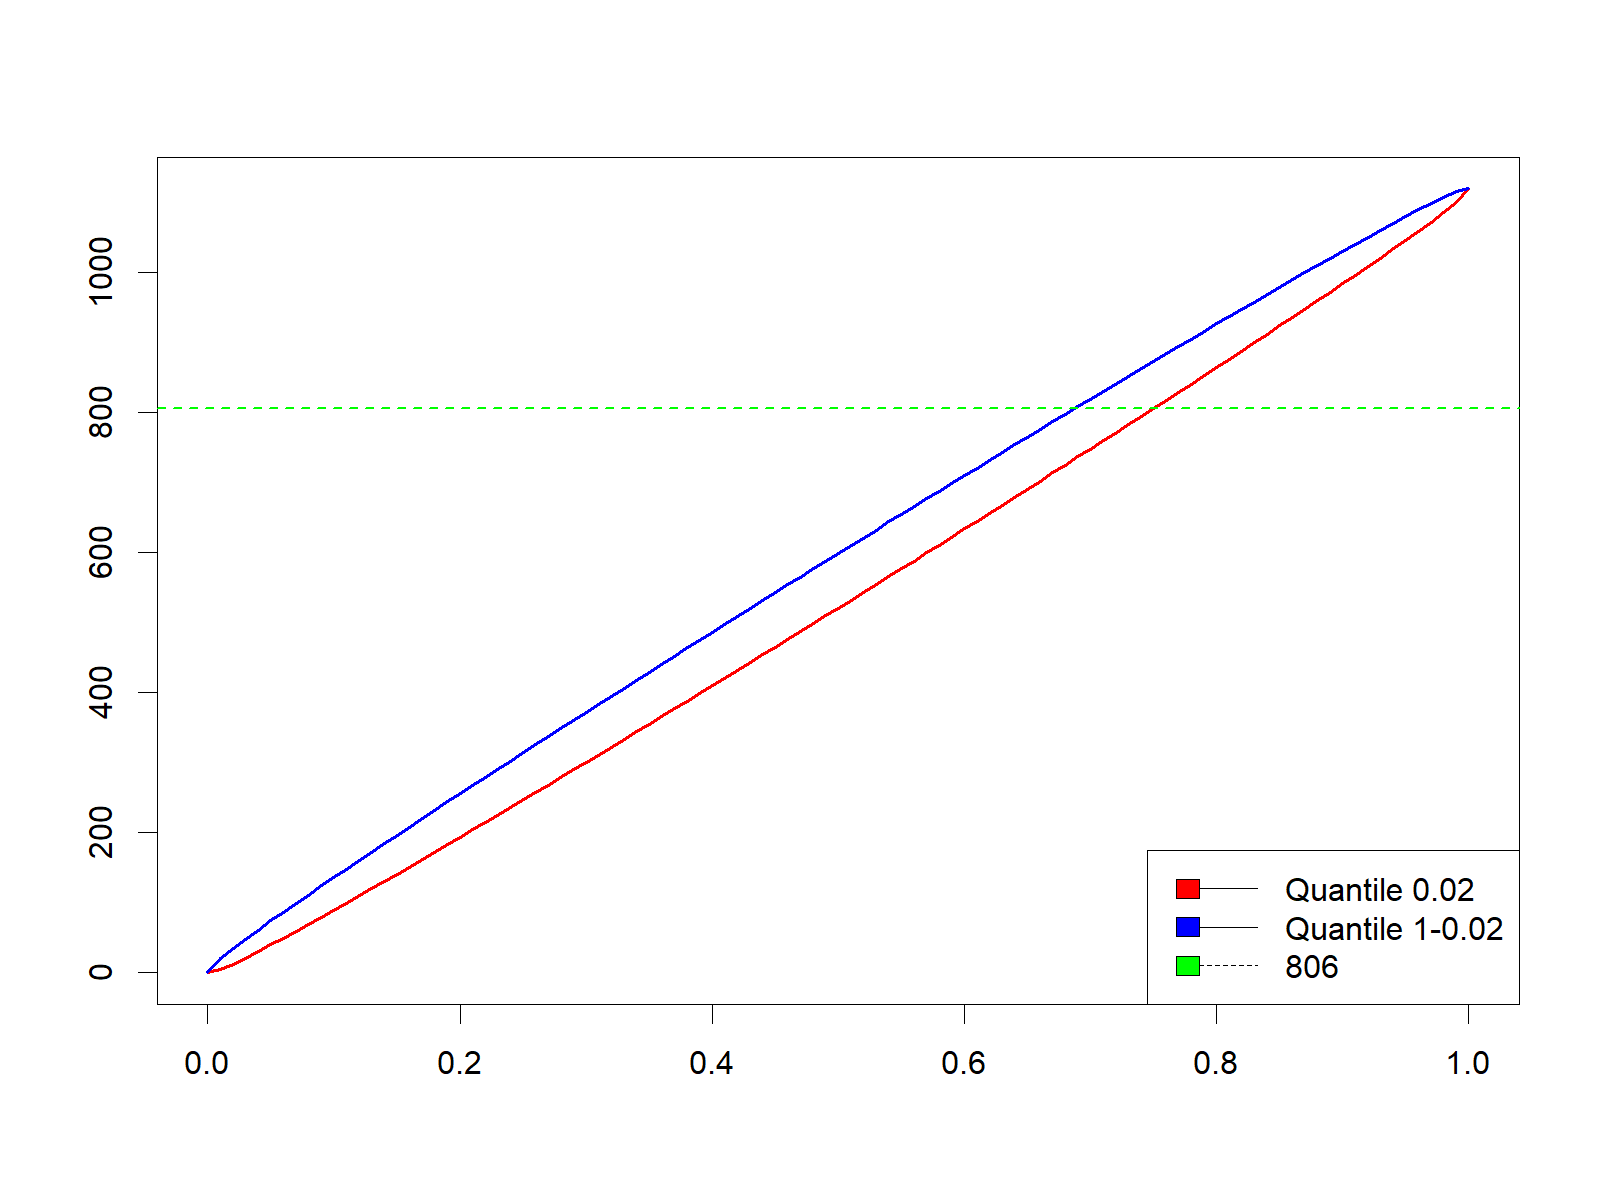
\includegraphics[width=0.7\linewidth]{../img/quantiles.png}}
\end{figure}
\begin{figure}[h]
	\centering{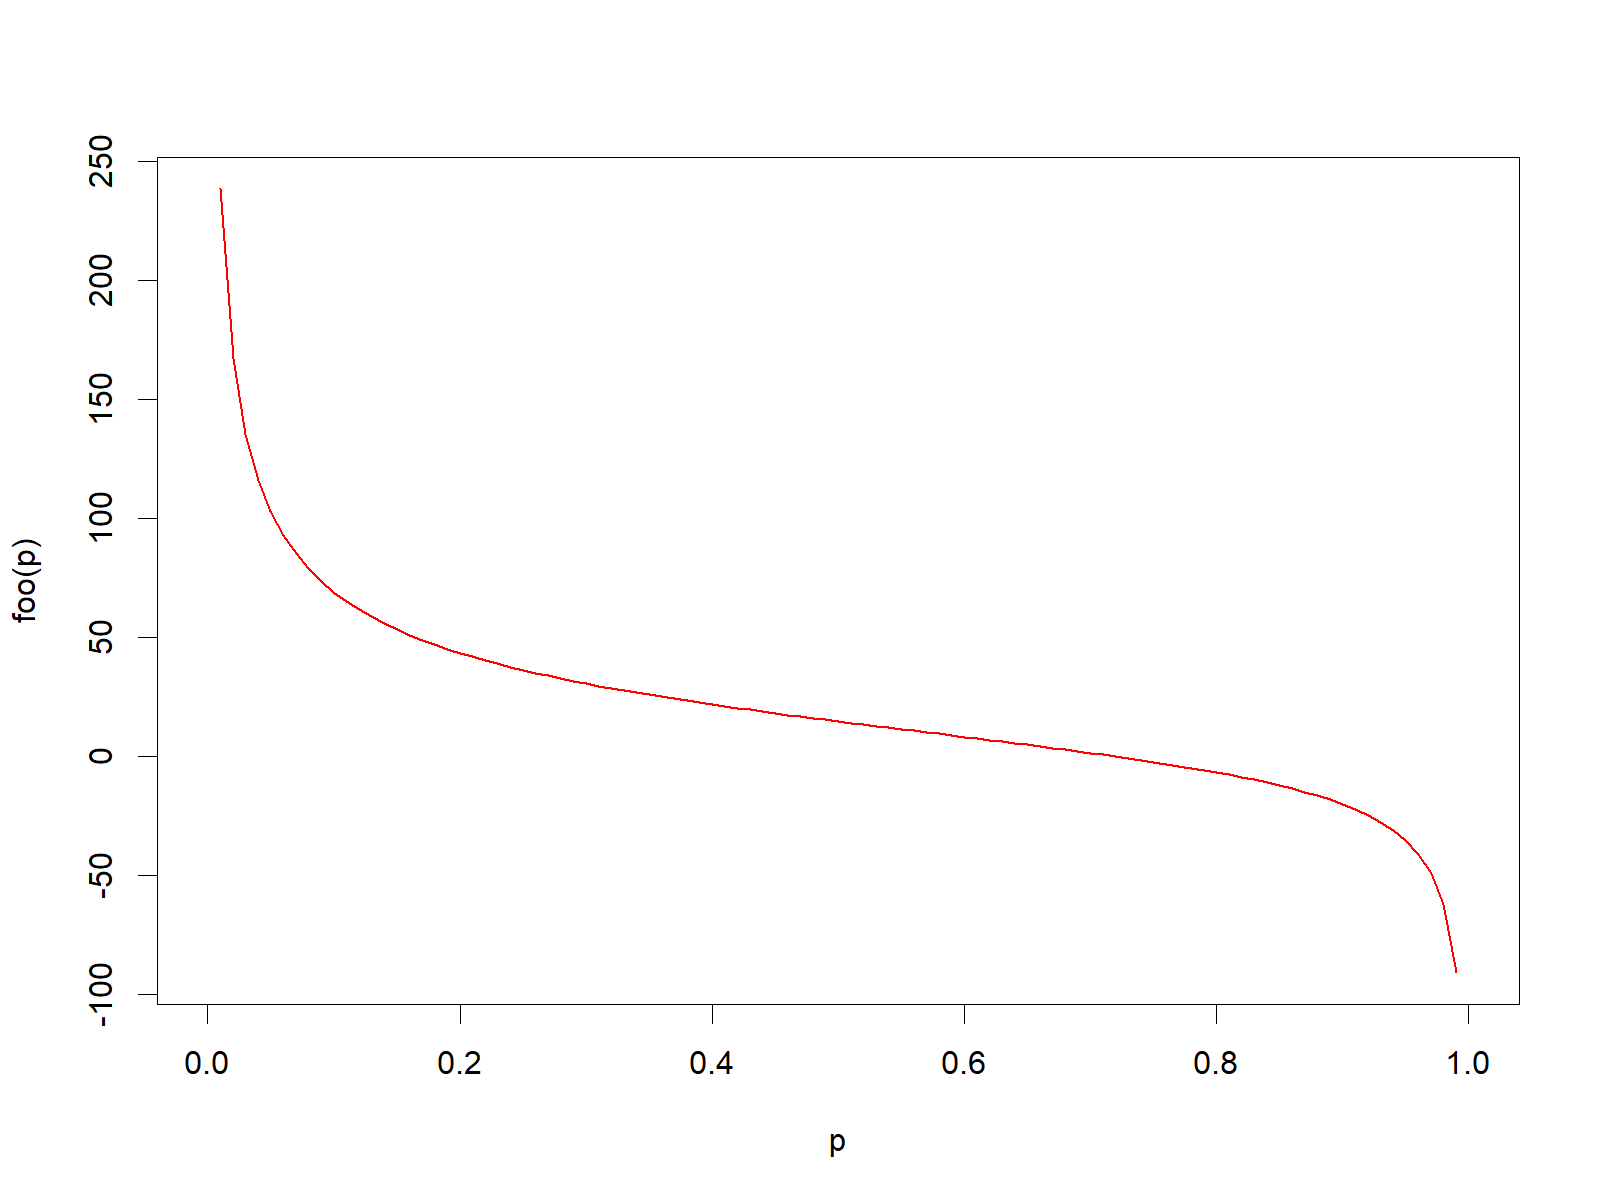
\includegraphics[width=0.7\linewidth]{../img/foo.png}}
\end{figure}

\newpage
Верхние и нижние оценки найдём из решений соответствующих уравнений:
\begin{minted}{R}
library(rootSolve)

clt_ci_LB.01_foo <- function(p) (sum(emp_sample) - n*k*p)/
(sqrt(n*k*p*(1-p))) - qnorm(1-0.1/2)
clt_ci_UB.01_foo <- function(p) (sum(emp_sample) - n*k*p)/
(sqrt(n*k*p*(1-p))) + qnorm(1-0.1/2)

clt_ci_LB.005_foo <- function(p) (sum(emp_sample) - n*k*p)/
(sqrt(n*k*p*(1-p))) - qnorm(1-0.05/2)
clt_ci_UB.005_foo <- function(p) (sum(emp_sample) - n*k*p)/
(sqrt(n*k*p*(1-p))) + qnorm(1-0.05/2)

clt_ci_LB.002_foo <- function(p) (sum(emp_sample) - n*k*p)/
(sqrt(n*k*p*(1-p))) - qnorm(1-0.02/2)
clt_ci_UB.002_foo <- function(p) (sum(emp_sample) - n*k*p)/
(sqrt(n*k*p*(1-p))) + qnorm(1-0.02/2)

clt_ci_LB.01 <- uniroot(clt_ci_LB.01_foo, c(0.1, 0.9))$root
clt_ci_UB.01 <- uniroot(clt_ci_UB.01_foo, c(0.1, 0.9))$root

clt_ci_LB.005 <- uniroot(clt_ci_LB.005_foo, c(0.1, 0.9))$root
clt_ci_UB.005 <- uniroot(clt_ci_UB.005_foo, c(0.1, 0.9))$root

clt_ci_LB.002 <- uniroot(clt_ci_LB.002_foo, c(0.1, 0.9))$root
clt_ci_UB.002 <- uniroot(clt_ci_UB.002_foo, c(0.1, 0.9))$root

clt_cis <- as.data.frame( matrix(c(clt_ci_LB.01, clt_ci_UB.01,
clt_ci_LB.005, clt_ci_UB.005,
clt_ci_LB.002, clt_ci_UB.002), 
byrow = T, ncol = 2))
colnames(clt_cis) <- c("Lower", "Upper")
rownames(clt_cis) <- c("0.1", "0.05", "0.02")

> clt_cis
alpha  Lower     Upper
0.1  0.6779266 0.7228906
0.05 0.6734280 0.7269840
0.02 0.6681609 0.7316903
\end{minted}

\section{Сравнение полученных результатов}
Сравним полученные в пп. \ref{sec1} и \ref{sec2} результаты для доверительных интервалов.\\
\textbf{Решение.}\\
\begin{minted}{R}
compare_CI <- as.data.frame(matrix(c(clt_ci_LB.01, cp_ci_LB.01, 
clt_ci_UB.01, cp_ci_UB.01,
clt_ci_LB.005, cp_ci_LB.005,
clt_ci_UB.005, cp_ci_UB.005,
clt_ci_LB.002, cp_ci_LB.002,
clt_ci_UB.002, cp_ci_UB.002), 
ncol = 2, byrow = T))
\end{minted}



\begin{table}[htbp]
	\centering
	\caption{CLT vs. CP CIs}
	\begin{tabular}{|c|c|c|c|}
		\hline
		alpha & CI    & V1    & V2 \bigstrut\\
		\hline
		\multirow{2}[4]{*}{alpha=0.1} & L     & 0.6779266 & 0.6775675 \bigstrut\\
		\cline{2-4}          & U     & 0.7228906 & 0.7234332 \bigstrut\\
		\hline
		\multirow{2}[4]{*}{alpha=0.05} & L     & 0.6734280 & 0.6731287 \bigstrut\\
		\cline{2-4}          & U     & 0.7269840 & 0.7275974 \bigstrut\\
		\hline
		\multirow{2}[4]{*}{alpha=0.02} & L     & 0.6681609 & 0.6679422 \bigstrut\\
		\cline{2-4}          & U     & 0.7316903 & 0.7324052 \bigstrut\\
		\hline
	\end{tabular}%
	\label{tab:addlabel}%
\end{table}%


Мы видим, что различия несущественные и все полученные интервалы содержат истинное значение параметра $p=0.7$.

\section{Построение CDF с CP CIs}
Для одного из значений $\alpha$ построим совмещённые графики функций распределения биномиальных законов $B(k,p)$, $B(k,\underline{p}), B(k,\bar{p})$. Рассмотрим $\alpha = 0.02$.
\begin{minted}{R}
theor_distr <- rbinom(n, k, p1)
distr_UB <- rbinom(n, k, cp_ci_UB.002)
distr_LB <- rbinom(n, k, cp_ci_LB.002)

plot(ecdf(theor_distr), 
col = "red", lwd = 3, verticals = T, axes = F,
xlim = c(0,k+1), ylim = c(0,1.2),
xlab = "Value", ylab = "CDF", main = "CDF with CIs")
plot(ecdf(distr_LB), 
col = "black", lwd = 2, verticals = T, add = T)
plot(ecdf(distr_UB), 
col = "blue", lwd = 2, verticals = T, add = T)
axis(1, c(1:k))
axis(2, seq(0.0, 1.2, 0.2), las = 1)
grid(nx = k+1, ny = 1.2 / 0.2)
legend("bottomright", c("Theoretical", "Lower", "Upper"), 
lty=c(1,1,1), 
fill=c("red", "black", "blue"))
\end{minted}

\begin{figure}[h]
	\centering{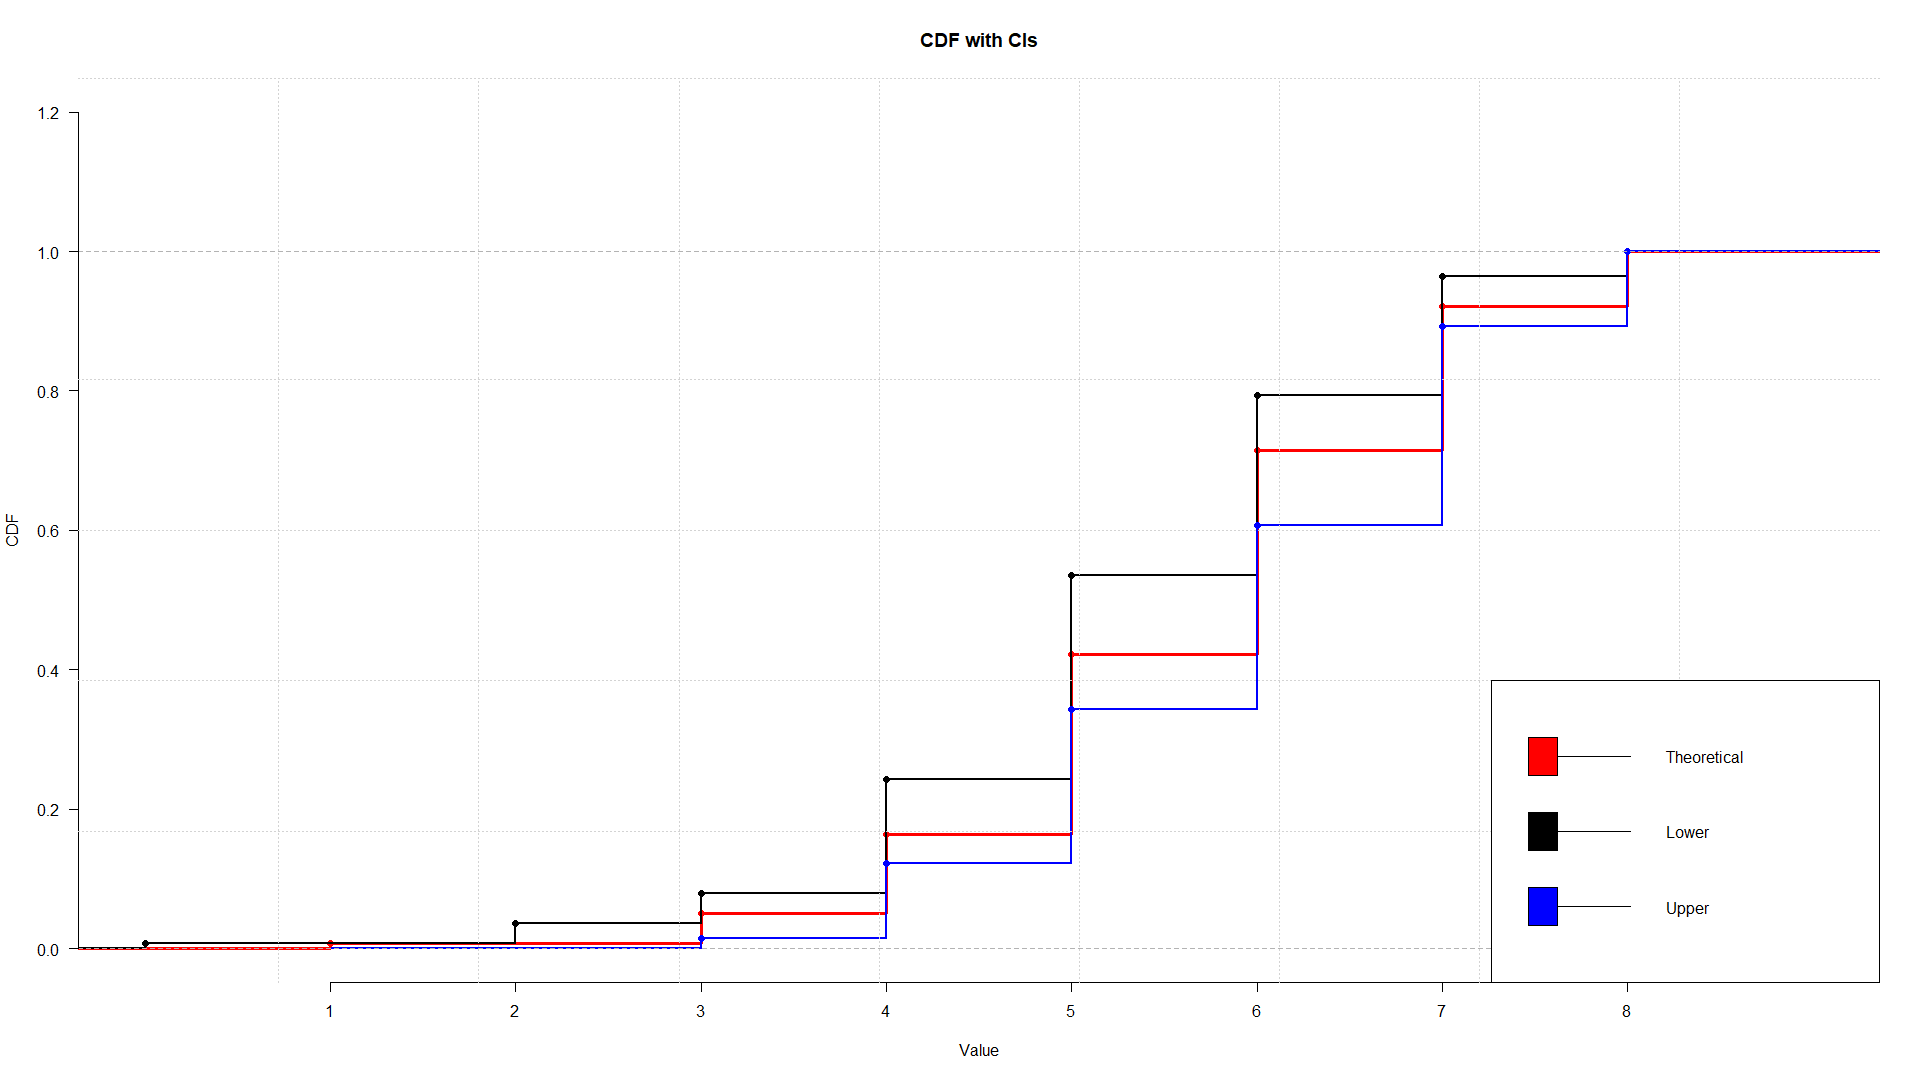
\includegraphics[width=1\linewidth]{../img/cdf_with_cis.png}}
\end{figure}




\end{document}